\documentclass{article}
\usepackage{kotex, verbatim}
\usepackage{amssymb,graphicx,verbatim,boxedminipage, subfigure,indentfirst}
\usepackage[left=2cm,right=2cm,top=2.54cm,bottom=2cm,a4paper]{geometry}
\usepackage[doublespacing]{setspace}

\title{프로그래밍 언어 hw4}
\author{B711016 김길호}
\date{\today}
\begin{document}
\maketitle
\newpage

\section{콜 그래프란?}
    콜 그래프란 하나의 프로그램을 구성하고 있는 단위 프로그램(함수, 프로시저)들 사이의 관계를 나타내는 그래프이며 그래프상에서 정점과 
    간선들로 표현됩니다. 이번 과제에서는 단위 프로그램이 함수명이므로 함수명이 정점이 되고, 정점들 간의 연결관계(라인 넘버, 호출 횟수)를 담는
    정보가 간선으로 표현됩니다.
    \begin{verbatim}
용어 참고 : https://terms.naver.com/entry.naver?docId=817069&cid=50376&categoryId=50376
    \end{verbatim}
\section{구현 설명}
    우선 설명에 앞서 과제 내용 중 일반 함수를 호출하며 콜 그래프를 구현하는 과정은 해냈으나, 포인터 함수를 구현하진 못했습니다. 이에 구현해낸 내용까지 서술하겠습니다. \\
    \subsection{설계 및 사용한 자료구조 설명}
        그래프를 모델링함에 있어서 어떤 자료구조를 쓸지부터 생각해봤습니다. 일단 함수들의 이름 자체로 정점의 인덱스를 표현할 수 없으므로 함수의 이름과 인덱스를 
        mapping시켜줄 2차원 CHAR배열 str2func을 선언한 뒤 map을 다루듯이 사용했고, 함수의 이름으로 인덱스를 구해야할 때 매번 str2func을 순회하며 인덱스를 구하기에 번거로워서 
        따로 함수를 작성해 인덱스를 반환해주는 query\_idx함수를 작성하였습니다.
        \begin{verbatim}
char str2func[MAX][21] ; // str2func[i] : key : str2func[i] , val : i   (for using map)
int query_idx(char *x){
        for (iter = 1; iter < funcidx; iter++)
            if (strcmp(x, str2func[iter]) == 0) 
                return iter;
        return -1;	
} 
        \end{verbatim}
        정점의 mapping문제를 해결한 뒤엔 간선들을 어떻게 표현할지 생각해봤습니다. 이번 과제에서 간선이 담는 정보는 line number와 사용 횟수였는데 이는
        정점(caller)과 정점(callee)사이에 line number들을 vector와 같은 자료구조에 담아놓는다면 해당 callee함수의 사용 횟수는 vector의 크기로 표현될 수 있었습니다.
        따라서 정점(caller)과 정점(callee)사이에 하나의 vector을 갖는 2차원 구조체를 선언하여 사용한다면 간선도 무리없이 표현할 수 있었고, vector구현체는 적절한 자료를 찾아
        사용하였습니다. 
        \newpage 
        \begin{verbatim}
/* vector 구현체 */
#define cvector_vector_type(type) type *
#define cvector_set_capacity(vec, size)     \
	do {                                    \
		if (vec) {                          \
			((size_t *)(vec))[-1] = (size); \
		}                                   \
	} while (0)


#define cvector_set_size(vec, size)         \
	do {                                    \
		if (vec) {                          \
			((size_t *)(vec))[-2] = (size); \
		}                                   \
	} while (0)


#define cvector_capacity(vec) \
	((vec) ? ((size_t *)(vec))[-1] : (size_t)0)


#define cvector_size(vec) \
	((vec) ? ((size_t *)(vec))[-2] : (size_t)0)


#define cvector_empty(vec) \
	(cvector_size(vec) == 0)

#define cvector_grow(vec, count)                                              \
	do {                                                                      \
		const size_t cv_sz = (count) * sizeof(*(vec)) + (sizeof(size_t) * 2); \
		if (!(vec)) {                                                         \
			size_t *cv_p = malloc(cv_sz);                                     \
			assert(cv_p);                                                     \
			(vec) = (void *)(&cv_p[2]);                                       \
			cvector_set_capacity((vec), (count));                             \
			cvector_set_size((vec), 0);                                       \
		} else {                                                              \
			size_t *cv_p1 = &((size_t *)(vec))[-2];                           \
			size_t *cv_p2 = realloc(cv_p1, (cv_sz));                          \
			assert(cv_p2);                                                    \
			(vec) = (void *)(&cv_p2[2]);                                      \
			cvector_set_capacity((vec), (count));                             \
		}                                                                     \
	} while (0)


#define cvector_pop_back(vec)                           \
	do {                                                \
		cvector_set_size((vec), cvector_size(vec) - 1); \
	} while (0)

#define cvector_erase(vec, i)                                  \
	do {                                                       \
		if (vec) {                                             \
			const size_t cv_sz = cvector_size(vec);            \
			if ((i) < cv_sz) {                                 \
				cvector_set_size((vec), cv_sz - 1);            \
				size_t cv_x;                                   \
				for (cv_x = (i); cv_x < (cv_sz - 1); ++cv_x) { \
					(vec)[cv_x] = (vec)[cv_x + 1];             \
				}                                              \
			}                                                  \
		}                                                      \
	} while (0)

#define cvector_free(vec)                        \
	do {                                         \
		if (vec) {                               \
			size_t *p1 = &((size_t *)(vec))[-2]; \
			free(p1);                            \
		}                                        \
	} while (0)

#define cvector_begin(vec) \
	(vec)

#define cvector_end(vec) \
	((vec) ? &((vec)[cvector_size(vec)]) : NULL)

#define cvector_push_back(vec, value)                               \
	do {                                                            \
		size_t cv_cap = cvector_capacity(vec);                      \
		if (cv_cap <= cvector_size(vec)) {                          \
			cvector_grow((vec), !cv_cap ? cv_cap + 1 : cv_cap * 2); \
		}                                                           \
		vec[cvector_size(vec)] = (value);                           \
		cvector_set_size((vec), cvector_size(vec) + 1);             \
	} while (0)

#define cvector_push_back(vec, value)                   \
	do {                                                \
		size_t cv_cap = cvector_capacity(vec);          \
		if (cv_cap <= cvector_size(vec)) {              \
			cvector_grow((vec), cv_cap + 1);            \
		}                                               \
		vec[cvector_size(vec)] = (value);               \
		cvector_set_size((vec), cvector_size(vec) + 1); \
	} while (0)

#define cvector_copy(from, to)									\
	do {														\
		for(size_t i = 0; i < cvector_size(from); i++) {		\
			cvector_push_back(to, from[i]);						\
		}														\
	} while (0)	
    												\
/* 하나의 vector를 담고있는 구조체선언 */
typedef struct EDGE{
    cvector_vector_type(int) l; 
} e;

e adj[MAX][MAX];  // adj[caller][callee].l : caller와 callee의 연결 관계를 담고있는 l벡터

/* 벡터 구현체 관련 참고 사이트 */
https://github.com/eteran/c-vector
        \end{verbatim}
        그래프 모델링을 끝낸 후엔 정점들을 순회하며 간선의 정보를 출력하도록 하는 간단한 그래프 순회 dfs 함수를 작성하였습니다. 
		이 때 방문하는 정점이 되기위한 필요충분조건은 정점의 이름이 함수 이름(func[])으로 체크되어 있어야하며, 정점간의 연결 관계를 담고있는 l벡터의 크기가 0이 아니여야합니다.
		또한 다음 방문할 정점은 현재의 정점과 다른 정점과 다른 경우에만 순회하도록 처리했습니다. (if (u != v) ~ 부분)
        \begin{verbatim}
void dfs(char *x){
        int u = query_idx(x), v;
        for (v = 1; v < funcidx; v++){
            if (func[v] == 0 || cvector_size(adj[u][v].l) == 0) continue;
            fprintf(graph, "\"%s\" -> \"%s\"", str2func[u], str2func[v]);
			            fprintf(graph, "[label=\"");
            fprintf(graph, "%d times line : ", cvector_size(adj[u][v].l));
            for (iter = 0; iter < cvector_size(adj[u][v].l); iter++){
                fprintf(graph, "%d ",adj[u][v].l[iter]);
            }
			            fprintf(graph, "\"]\n");
            if (u != v) dfs(str2func[v]);
        }
}
        \end{verbatim}
    \subsection{lex, yacc 수정사항}
        정점간의 연결 관계에 라인 넘버가 간선의 정보로 들어가므로 lex에서 현재 보고있는 라인 넘버를 관리해야했습니다. 이는
        yacc에서 현재 라인의 정보를 담을 변수 line을 선언하였고, lex내에서 extern으로 선언하였습니다. line이 바뀌는(개행이 일어나는) 상황은 
        주석 처리하는 부분에서 발생하는 개행, lex에서 정한 토큰들에 걸리지않고 개행, inclue define과 같은 전처리문
        에서의 개행으로 총 세 가지 경우가 존재했고, 개행이 나타날 때마다 line을 증가시켜 yacc에서 현재 보는 함수의 라인 넘버를 정확하게
        알 수 있었습니다. 함수의 이름을 받아오는 과정은 yacc에서 char형 배열 name[]을 선언하고, lex에서 line과 비슷한 방식으로 
        IDENTIFIER가 매칭될 때마다 name에 yytext를 복사해 yacc에서 현재 보고있는 IDENTIFIER을 알 수 있었습니다.  
        \begin{verbatim}
/* lex 수정 부분 */
<COMMENT>.|\n	{if(strcmp(yytext,"\n") == 0) line++;}
"\n" {line++;}
        \end{verbatim}
        마지막으로 남은 것은 IDENTIFIER에서 각기 다르게 reduce되는 함수 이름을 어떻게 파싱할지가 문제였습니다. 함수 이름을 저장해야 하는 경우를 따져본다면 
        사용자 정의 함수는 정의를 해야 사용 할 수 있기에 함수를 정의할 때 함수 이름을 저장해주면 된다고 생각했고, printf, scanf와 같은 내장 함수는 따로 정의하지않고 
        사용할 수 있었기에 이에 대한 별도의 처리를 해주어 해결하였습니다. 따라서 함수의 이름 저장하는 과정에서 사용한 용어를 정리한 후, 두 경우를 나눠서 서술하겠습니다. \\
            \subsubsection{용어 정의}
            	caller[] : 정의된 함수 이름을 담아놓는 임시 배열\\
                callee[] : printf, scanf와 같이 정의되지 않고 사용되는 내장 함수의 이름을 담아놓는 임시 배열\\
                func[idx] : query\_idx함수로 반환한 인덱스 값에 해당하는 이름의 변수가 함수의 이름인지 체크하는 배열\\
                isfunc : 함수를 정의, 사용하는 과정에서의 체크 변수\\

            \subsubsection{함수를 정의할 때 이름을 저장}
                함수를 정의할 때 이름은 function\_definition에서 정보를 저장해주면 되었고, 이를 위해 몇 가지 과정을 거쳤습니다.\\
                1. 함수 정의 과정에서 함수의 이름은 IDENTIFIER에서 direct\_declarator으로 reduce되기 때문에 함수 이름을 담아줄 caller가 비어있다면 name을 caller에 넣어줍니다.\\
                2. 단순 변수 선언문도 IDENTIFIER에서 direct\_declarator으로 reduce되기 때문에 정확히 함수가 정의되는 경우에만 함수의 이름으로 저장하기 위해 isfunc변수를 사용하여 function\_definition으로 reduce되기 전
                   isfunc변수를 체크해줬습니다.\\
                3. function\_definition에서 external\_declaration으로 reduce되기전 query\_idx함수로 caller의 인덱스가 없다면 str2func배열에 caller을 저장하고, 함수 인덱스를 cur에 담아준 뒤 
				   불러와 func[cur]에 체크를 해뒀습니다. 또한 선언이 끝났기에 caller와 infunc를 초기화해줬습니다.
			\newpage
			\begin{verbatim}
direct_declarator
	: IDENTIFIER {
		// Save caller name (func name)
        if (isempty(caller)) {
            strcpy(caller,name);
            cur = query_idx(caller);
            if (cur < 0){
                strcpy(str2func[funcidx], caller);
                cur = funcidx;
                funcidx++;
            }
        }
    }

external_declaration 
	: function_definition{
        cur = query_idx(caller);
        if (cur < 0){
                strcpy(str2func[funcidx], caller);
                cur = funcidx;
                funcidx++;
		}
        if (isfunc) func[cur] = 1;
        strcpy(caller,"");
        isfunc = 0;
    }
			\end{verbatim}

            \subsubsection{내장 함수를 사용할 때 이름을 저장}
                내장 함수의 경우 내장 함수를 정의하지 않고 사용할 수 있고, 항상 다른 함수안에서 사용되었기에 printf, scanf와 같은 함수의 이름을 담아두기전 caller가 담겨져있었습니다. (다른 함수안에서 사용되었기에) 
				따라서 이와 같은 내장함수의 이름을 저장할 때는 caller에 저장하는 것이 아니라 callee가 비어있는 경우에만 IDENTIFIER에서 primary\_expression으로 reduce되기 전 callee에 담아주었습니다.
				이제 내장 함수의 이름이 callee에 담겨있으니 postfix\_expression '(' ')' 에서  postfix\_expression, postfix\_expression '(' argument\_expression\_list ')' 에서 postfix\_expression으로
				reduce되기전 함수 사용을 했다는 의미에서 isfunc체크를 해준 후, expression ';' 에서 expression\_statement으로 reduce될 때 isfunc이 체크된 경우에만 caller와의 연결 관계를 연결해주면 함수 이름 
				func[]체크뿐만아니라 앞서 선언된 함수(caller)와 연결해줄 수 있었습니다. 또한 return 문에서 내장 함수를 사용할 때도 같은 방식으로 처리할 수 있었습니다. 하지만 이는 caller와 callee의 관계만 연결할 뿐 
                아래 사진의 예시처럼 caller와 함수안에 들어있는 함수까지 연결 관계를 표현할 수 없었기에 아래와 같이 해결하였습니다. \\  
				\begin{figure}[h]
					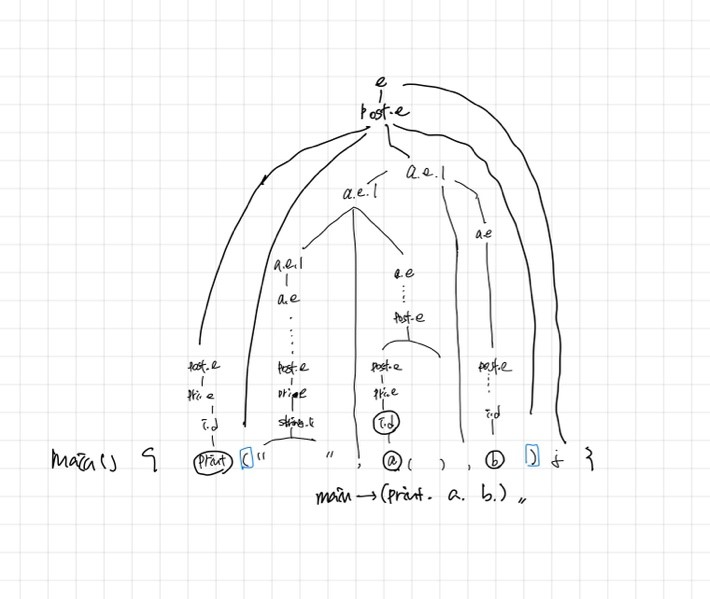
\includegraphics[width = 0.6\textwidth]{func.jpg}
				\end{figure}
				\\1. IDENTIFIER에서 primary\_expression으로 reduce되기 전 callee저장과 별개로 caller와 현재 IDENTIFIER으로 받아온 name을 연결, name을 str2func에 저장해줍니다. 
				\\	 (caller와 모든 name과 연결하는 이유는 단순 변수명이든 함수명이든 IDENTIFIER로 인식되기 때문에 IDENTIFIER에서 primary\_expression으로 reduce되는 순간엔 그 name이 함수인지 변수인지 알지 못해서
				      우선 연결해둡니다.)\\
				  2. 모든 name과 연결하였기에 main부터 순회를 할 때, 함수 이름이 아닌 변수 이름을 탐색할 수도 있을 것 같지만 dfs돌리는 과정에서 항상 func[]체크된 정점만 방문하기에 모든 name과 연결해두더라도
				     항상 함수 이름 정점만 방문하며 순회할 수 있습니다.
			\begin{verbatim}
primary_expression
	: IDENTIFIER {
			cur = query_idx(caller);
            if (cur < 0){
                strcpy(str2func[funcidx], caller);
                cur = funcidx;
                funcidx++;                
            }
            func[cur] = 1;

			if (isempty(callee)) strcpy(callee, name);
			nxt = query_idx(name);
			if (nxt < 0){
				strcpy(str2func[funcidx], name);
				nxt = funcidx;
				funcidx++;
			}
			cvector_push_back(adj[cur][nxt].l, line);
    }
	
expression_statement
	| expression ';'{
			nxt = query_idx(callee);
			if (nxt < 0){
				strcpy(str2func[funcidx], callee);
				nxt = funcidx;
				funcidx++;
			}
			if(isfunc) func[nxt] = 1; 
			isfunc=0;
			strcpy(callee, "");
        }
	;

jump_statement
	| RETURN expression ';'{
			nxt = query_idx(callee);
			if (nxt < 0){
				strcpy(str2func[funcidx], callee);
				nxt = funcidx;
				funcidx++;
			}
			if(isfunc) func[nxt] = 1; 
			isfunc=0;
			strcpy(callee, "");
        }
	;
			\end{verbatim}

			\subsubsection{yacc내 main함수 부분과 앞서 언급하지 않은 부분}
			1. main에선 선언한 구조체 배열내의 벡터를 NULL로 초기화해주었고, 실습 시간에 다뤘던 dot명령어를 사용해 gv파일을 jpg파일로 생성했습니다.\\
			2. 2차원 구조체 adj를 선언할 때나 함수 관련 배열을 선언할 때, 크기를 2001정도로 지정해 선언했는데 이는 테스트케이스에서 함수가 몇개 정도 선언될 지 모르는 상태이기에 적당한 크기로 지정했습니다.\\
			3. IDENTIFIER에서 primary\_expression으로 reduce되기 전 callee가 비어있으면 callee에 담았는데 변수 선언, 값 배정과 같이 함수 이름이 아닌 변수가 callee에 담겨 caller와 연결되는 걸 막기위해서 각각 해당되는 부분에 callee를 적절하게 빈 문자열로 초기화해줬습니다.

			\newpage
			\section{Yacc 구현 코드}
\begin{verbatim}
%{
#include <stdio.h>
#include <string.h>
#include <assert.h> /* for assert */
#include <stdlib.h> /* for malloc/realloc/free */

#define MAX 2001
char name[21] = "", caller[21]= "", callee[21] = "";

char str2func[MAX][21], pfunc[MAX][21], ptr2func[MAX][21];
// str2func[i] : key : str2func[i] , val : i   (for using map)
// ptr2func[i] : key : ptr2func[i] , val : i   (for using map)
// pfunc[i] : ptr2func[i]이 가리키는 함수

int isfunc = 0, func[MAX];
int funcidx = 1, ptrfuncidx = 1, ptrfunc = 0, line = 1;
int cur, nxt;
int iter, iter2, iter3;

#define cvector_vector_type(type) type *

#define cvector_set_capacity(vec, size)     \
	do {                                    \
		if (vec) {                          \
			((size_t *)(vec))[-1] = (size); \
		}                                   \
	} while (0)


#define cvector_set_size(vec, size)         \
	do {                                    \
		if (vec) {                          \
			((size_t *)(vec))[-2] = (size); \
		}                                   \
	} while (0)


#define cvector_capacity(vec) \
	((vec) ? ((size_t *)(vec))[-1] : (size_t)0)


#define cvector_size(vec) \
	((vec) ? ((size_t *)(vec))[-2] : (size_t)0)


#define cvector_empty(vec) \
	(cvector_size(vec) == 0)

#define cvector_grow(vec, count)                                              \
	do {                                                                      \
		const size_t cv_sz = (count) * sizeof(*(vec)) + (sizeof(size_t) * 2); \
		if (!(vec)) {                                                         \
			size_t *cv_p = malloc(cv_sz);                                     \
			assert(cv_p);                                                     \
			(vec) = (void *)(&cv_p[2]);                                       \
			cvector_set_capacity((vec), (count));                             \
			cvector_set_size((vec), 0);                                       \
		} else {                                                              \
			size_t *cv_p1 = &((size_t *)(vec))[-2];                           \
			size_t *cv_p2 = realloc(cv_p1, (cv_sz));                          \
			assert(cv_p2);                                                    \
			(vec) = (void *)(&cv_p2[2]);                                      \
			cvector_set_capacity((vec), (count));                             \
		}                                                                     \
	} while (0)


#define cvector_pop_back(vec)                           \
	do {                                                \
		cvector_set_size((vec), cvector_size(vec) - 1); \
	} while (0)

#define cvector_erase(vec, i)                                  \
	do {                                                       \
		if (vec) {                                             \
			const size_t cv_sz = cvector_size(vec);            \
			if ((i) < cv_sz) {                                 \
				cvector_set_size((vec), cv_sz - 1);            \
				size_t cv_x;                                   \
				for (cv_x = (i); cv_x < (cv_sz - 1); ++cv_x) { \
					(vec)[cv_x] = (vec)[cv_x + 1];             \
				}                                              \
			}                                                  \
		}                                                      \
	} while (0)

#define cvector_free(vec)                        \
	do {                                         \
		if (vec) {                               \
			size_t *p1 = &((size_t *)(vec))[-2]; \
			free(p1);                            \
		}                                        \
	} while (0)

#define cvector_begin(vec) \
	(vec)

#define cvector_end(vec) \
	((vec) ? &((vec)[cvector_size(vec)]) : NULL)

#define cvector_push_back(vec, value)                               \
	do {                                                            \
		size_t cv_cap = cvector_capacity(vec);                      \
		if (cv_cap <= cvector_size(vec)) {                          \
			cvector_grow((vec), !cv_cap ? cv_cap + 1 : cv_cap * 2); \
		}                                                           \
		vec[cvector_size(vec)] = (value);                           \
		cvector_set_size((vec), cvector_size(vec) + 1);             \
	} while (0)

#define cvector_push_back(vec, value)                   \
	do {                                                \
		size_t cv_cap = cvector_capacity(vec);          \
		if (cv_cap <= cvector_size(vec)) {              \
			cvector_grow((vec), cv_cap + 1);            \
		}                                               \
		vec[cvector_size(vec)] = (value);               \
		cvector_set_size((vec), cvector_size(vec) + 1); \
	} while (0)

#define cvector_copy(from, to)									\
	do {														\
		for(size_t i = 0; i < cvector_size(from); i++) {		\
			cvector_push_back(to, from[i]);						\
		}														\
	} while (0)													\

int query_idx(char *x){
	for (iter = 1; iter < funcidx; iter++)
		if (strcmp(x, str2func[iter]) == 0) 
			return iter;
	return -1;	
}

int query_ptr_idx(char *x){
	for (iter = 1; iter < ptrfuncidx; iter++)
		if (strcmp(x, ptr2func[iter]) == 0) 
			return iter;
	return -1;	
}

int isempty(char *x){
	if (strlen(x) == 0) return 1;
	return 0;
}


typedef struct EDGE{
    cvector_vector_type(int) l;
} e;

e adj[MAX][MAX];
FILE * graph;

void dfs(char *x){
    int u = query_idx(x), v;
    for (v = 1; v < funcidx; v++){
            if (func[v] == 0 || cvector_size(adj[u][v].l) == 0) continue;
            fprintf(graph, "\"%s\" -> \"%s\"", str2func[u], str2func[v]);
			fprintf(graph, "[label=\"");
            fprintf(graph, "%d times line : ", cvector_size(adj[u][v].l));
            for (iter = 0; iter < cvector_size(adj[u][v].l); iter++){
                fprintf(graph, "%d ",adj[u][v].l[iter]);
            }
			fprintf(graph, "\"]\n");
            if (u != v) dfs(str2func[v]);
        }
}

%}

%token IDENTIFIER CONSTANT STRING_LITERAL SIZEOF
%token PTR_OP INC_OP DEC_OP LEFT_OP RIGHT_OP LE_OP GE_OP EQ_OP NE_OP
%token AND_OP OR_OP MUL_ASSIGN DIV_ASSIGN MOD_ASSIGN ADD_ASSIGN
%token SUB_ASSIGN LEFT_ASSIGN RIGHT_ASSIGN AND_ASSIGN
%token XOR_ASSIGN OR_ASSIGN TYPE_NAME

%token TYPEDEF EXTERN STATIC AUTO REGISTER
%token CHAR SHORT INT LONG SIGNED UNSIGNED FLOAT DOUBLE CONST VOLATILE VOID
%token STRUCT UNION ENUM ELLIPSIS

%token CASE DEFAULT IF ELSE SWITCH WHILE DO FOR GOTO CONTINUE BREAK RETURN
%nonassoc LOWER_THEN_ELSE
%nonassoc ELSE
%start translation_unit
%%

primary_expression
	: IDENTIFIER {
			cur = query_idx(caller);
            if (cur < 0){
                strcpy(str2func[funcidx], caller);
                cur = funcidx;
                funcidx++;                
            }
            func[cur] = 1;

			if (isempty(callee)) strcpy(callee, name);
			nxt = query_idx(name);
			if (nxt < 0){
				strcpy(str2func[funcidx], name);
				nxt = funcidx;
				funcidx++;
			}
			cvector_push_back(adj[cur][nxt].l, line);
    }
	| CONSTANT 
	| STRING_LITERAL 
	| '(' expression ')' 
	;

postfix_expression
	: primary_expression 
	| postfix_expression '[' expression ']' 
	| postfix_expression '(' ')' {isfunc = 1;}
	| postfix_expression '(' argument_expression_list ')' {isfunc = 1;}
	| postfix_expression '.' IDENTIFIER 
	| postfix_expression PTR_OP IDENTIFIER
	| postfix_expression INC_OP 
	| postfix_expression DEC_OP 
	;

argument_expression_list
	: assignment_expression
	| argument_expression_list ',' assignment_expression 
	;

unary_expression
	: postfix_expression 
	| INC_OP unary_expression 
	| DEC_OP unary_expression 
	| unary_operator cast_expression   
	| SIZEOF unary_expression  
	| SIZEOF '(' type_name ')'
	;

unary_operator
	: '&'
	| '*'
	| '+'
	| '-'
	| '~'
	| '!'
	;

cast_expression
	: unary_expression 
	| '(' type_name ')' cast_expression 
	;

multiplicative_expression
	: cast_expression 
	| multiplicative_expression '*' cast_expression 
	| multiplicative_expression '/' cast_expression 
	| multiplicative_expression '%' cast_expression 
	;

additive_expression
	: multiplicative_expression
	| additive_expression '+' multiplicative_expression 
	| additive_expression '-' multiplicative_expression 
	;

shift_expression
	: additive_expression
	| shift_expression LEFT_OP additive_expression		
	| shift_expression RIGHT_OP additive_expression		
	;

relational_expression
	: shift_expression
	| relational_expression '<' shift_expression 	
	| relational_expression '>' shift_expression 	
	| relational_expression LE_OP shift_expression 
	| relational_expression GE_OP shift_expression 
	;

equality_expression
	: relational_expression
	| equality_expression EQ_OP relational_expression 	
	| equality_expression NE_OP relational_expression 	
	;

and_expression
	: equality_expression
	| and_expression '&' equality_expression 	
	;

exclusive_or_expression
	: and_expression
	| exclusive_or_expression '^' and_expression 	
	;

inclusive_or_expression
	: exclusive_or_expression
	| inclusive_or_expression '|' exclusive_or_expression 	
	;

logical_and_expression
	: inclusive_or_expression
	| logical_and_expression AND_OP inclusive_or_expression 
	;

logical_or_expression
	: logical_and_expression
	| logical_or_expression OR_OP logical_and_expression 	
	;

conditional_expression
	: logical_or_expression
	| logical_or_expression '?' expression ':' conditional_expression
	;

assignment_expression
	: conditional_expression 
	| unary_expression assignment_operator assignment_expression 
	;

assignment_operator
	: '=' {
		// 포인터함수 고친다면 여기서
		strcpy(callee, "");
	}
	| MUL_ASSIGN
	| DIV_ASSIGN
	| MOD_ASSIGN
	| ADD_ASSIGN
	| SUB_ASSIGN
	| LEFT_ASSIGN
	| RIGHT_ASSIGN
	| AND_ASSIGN
	| XOR_ASSIGN
	| OR_ASSIGN
	;

expression
	: assignment_expression{
		if (isfunc == 0) strcpy(callee,"");
    }
	| expression ',' assignment_expression{
		if (isfunc == 0) strcpy(callee,"");
    }
	;

constant_expression
	: conditional_expression 
	;

declaration
	: declaration_specifiers ';' {strcpy(callee, "");}
	| declaration_specifiers init_declarator_list ';' {strcpy(callee, "");}
	;

declaration_specifiers
	: storage_class_specifier declaration_specifiers 
	| storage_class_specifier
	| type_specifier declaration_specifiers 
	| type_specifier 
	| type_qualifier declaration_specifiers
	| type_qualifier 
	;

init_declarator_list
	: init_declarator 
	| init_declarator_list ',' init_declarator
	;

init_declarator
	: declarator 
	| declarator '=' initializer  
	;

storage_class_specifier
	: TYPEDEF 
	| EXTERN 
	| STATIC 
	| AUTO
	| REGISTER 
	;

type_specifier
	: VOID 
	| CHAR 
	| SHORT 
	| INT 
	| LONG 
	| FLOAT 
	| DOUBLE 
	| SIGNED 
	| UNSIGNED 
	| struct_or_union_specifier 
	| enum_specifier 
	| TYPE_NAME 
	;

struct_or_union_specifier
	: struct_or_union '{' struct_declaration_list '}' 
	| struct_or_union IDENTIFIER '{' struct_declaration_list '}' 
	| struct_or_union IDENTIFIER 
	;

struct_or_union
	: STRUCT 
	| UNION 
	;

struct_declaration_list
	: struct_declaration 
	| struct_declaration_list struct_declaration 
	;

struct_declaration
	: specifier_qualifier_list struct_declarator_list ';' 
	;

specifier_qualifier_list
	: type_specifier specifier_qualifier_list 
	| type_specifier 
	| type_qualifier specifier_qualifier_list 
	| type_qualifier 
	;

struct_declarator_list
	: struct_declarator 
	| struct_declarator_list ',' struct_declarator 
	;

struct_declarator
	: declarator 
	| ':' constant_expression 
	| declarator ':' constant_expression 
	;

enum_specifier
	: ENUM '{' enumerator_list '}'
	| ENUM IDENTIFIER '{' enumerator_list '}'
	| ENUM IDENTIFIER
	;

enumerator_list
	: enumerator
	| enumerator_list ',' enumerator
	;

enumerator
	: IDENTIFIER
	| IDENTIFIER '=' constant_expression 
	;

type_qualifier
	: CONST
	| VOLATILE
	;

declarator
	: pointer direct_declarator {ptrfunc = 1;}
	| direct_declarator 
	;

direct_declarator
	: IDENTIFIER {
		// Save caller name (func name)
        if (isempty(caller)) {
            strcpy(caller,name);
            cur = query_idx(caller);
            if (cur < 0){
                strcpy(str2func[funcidx], caller);
                cur = funcidx;
                funcidx++;
            }
        }
    }
	| '(' declarator ')' {
        if (ptrfunc){
			/* save func ptr name*/
            cur = query_idx(caller);
            if (cur < 0){
                strcpy(str2func[funcidx], caller);
                cur = funcidx;
                funcidx++;                
            }
            func[cur] = 1;

            nxt = query_ptr_idx(name);
			if (nxt < 0){
				strcpy(ptr2func[ptrfuncidx], name);
				//printf("######ptr func : %s\n",ptr2func[ptrfuncidx]);
                nxt = ptrfuncidx;
                // connect caller <-> ptr func
				ptrfuncidx++;
			}
        }
        ptrfunc = 0;
    }
	| direct_declarator '[' constant_expression ']' 
	| direct_declarator '[' ']' 
	| direct_declarator '(' parameter_type_list ')' 
	| direct_declarator '(' identifier_list ')'  
	| direct_declarator '(' ')'  
	;

pointer
	: '*'
	| '*' type_qualifier_list
	| '*' pointer
	| '*' type_qualifier_list pointer
	;

type_qualifier_list
	: type_qualifier
	| type_qualifier_list type_qualifier
	;


parameter_type_list
	: parameter_list 
	| parameter_list ',' ELLIPSIS
	;

parameter_list
	: parameter_declaration 
	| parameter_list ',' parameter_declaration 
	;

parameter_declaration
	: declaration_specifiers declarator
	| declaration_specifiers abstract_declarator 
	| declaration_specifiers 
	;

identifier_list
	: IDENTIFIER 
	| identifier_list ',' IDENTIFIER 
	;

type_name
	: specifier_qualifier_list
	| specifier_qualifier_list abstract_declarator
	;

abstract_declarator
	: pointer
	| direct_abstract_declarator
	| pointer direct_abstract_declarator
	;

direct_abstract_declarator
	: '(' abstract_declarator ')'
	| '[' ']'
	| '[' constant_expression ']'
	| direct_abstract_declarator '[' ']'
	| direct_abstract_declarator '[' constant_expression ']'
	| '(' ')'
	| '(' parameter_type_list ')'
	| direct_abstract_declarator '(' ')'
	| direct_abstract_declarator '(' parameter_type_list ')'
	;

initializer
	: assignment_expression
	| '{' initializer_list '}'
	| '{' initializer_list ',' '}'
	;

initializer_list
	: initializer
	| initializer_list ',' initializer
	;

statement
	: labeled_statement {strcpy(callee, "");}
	| compound_statement {strcpy(callee, "");}
	| expression_statement {strcpy(callee, "");}
	| selection_statement {strcpy(callee, "");}
	| iteration_statement {strcpy(callee, "");}
	| jump_statement {strcpy(callee, "");}
	;

labeled_statement
	: IDENTIFIER ':' statement
	| CASE constant_expression ':' statement
	| DEFAULT ':' statement
	;

compound_statement
	: '{' '}'
	| '{'  block_item_list '}'
	;

block_item_list
	: block_item
	| block_item_list block_item
	;

block_item
	: declaration
	| statement
	;

expression_statement
	: ';'
	| expression ';'{
			nxt = query_idx(callee);
			if (nxt < 0){
				strcpy(str2func[funcidx], callee);
				nxt = funcidx;
				funcidx++;
			}
			if(isfunc) func[nxt] = 1; 
			isfunc=0;
			strcpy(callee, "");
        }
	;

selection_statement
	: IF '(' expression ')' statement %prec LOWER_THEN_ELSE 	
	| IF '(' expression ')' statement ELSE statement			
	| SWITCH '(' expression ')' statement 						
	;

iteration_statement
	: WHILE '(' expression ')' statement	
	| DO statement WHILE '(' expression ')' ';' 
	| FOR '(' expression_statement expression_statement ')' statement
	| FOR '(' expression_statement expression_statement expression ')' statement  
	| FOR '(' declaration expression_statement ')' statement 
	| FOR '(' declaration expression_statement expression ')' statement  
	;

jump_statement
	: GOTO IDENTIFIER ';'
	| CONTINUE ';'
	| BREAK ';'
	| RETURN ';'  
	| RETURN expression ';'{
			nxt = query_idx(callee);
			if (nxt < 0){
				strcpy(str2func[funcidx], callee);
				nxt = funcidx;
				funcidx++;
			}
			if(isfunc) func[nxt] = 1; 
			isfunc=0;
			strcpy(callee, "");
        }
	;

translation_unit
	: external_declaration
	| translation_unit external_declaration
	;

external_declaration 
	: function_definition{
        cur = query_idx(caller);
        if (cur < 0){
                strcpy(str2func[funcidx], caller);
                cur = funcidx;
                funcidx++;
		}
        if (isfunc) func[cur] = 1;
        strcpy(caller,"");
        isfunc = 0;
    }
	| declaration{
    	strcpy(caller, "");
		strcpy(callee, "");
    }
	;

function_definition
	: declaration_specifiers declarator declaration_list compound_statement 
	| declaration_specifiers declarator compound_statement 
	| declarator declaration_list compound_statement 
	| declarator compound_statement 
	;

declaration_list
	: declaration
	| declaration_list declaration
	;

%%

int main(void){
    for (iter = 0 ; iter < MAX; iter++){
        for (iter2 = 0; iter2 < MAX; iter2++){
            adj[iter][iter2].l = NULL;
        }
    }
	yyparse();
	graph = fopen("B711016.gv","w");
	fprintf(graph,"digraph{\n");
    fprintf(graph,"edge [color=black]\n");
    dfs("main");
	fprintf(graph,"}");
	fclose(graph);
    system("dot -Tjpg B711016.gv -o B711016.jpg");
	return 0;
}

void yyerror(const char *str)
{
	fprintf(stderr, "error: %s\n", str);
}

\end{verbatim}
\end{document}
